\section{(Protein-) Strukturvorhersage (3D)}
\subsection{Strukturaufklärung}
\begin{itemize}
  \item Röntgen-Kristallographie
  \item NMR
\end{itemize}
\subsection{Qualität der Strukturvorhersage}
\begin{itemize}
\item RMSD (root mean square deviation): mittlerer Abstand in \AA{} (10\textsuperscript{-10} m)
\end{itemize}
1-2 \AA{} RMSD ist ein (sehr) guter Wert.
\subsection{Problem der Strukturvorhersage (Levinthal-Paradoxon)}
Eine Polypeptidkette von 100 Residuen hat 99 Peptidbindungen und daher 198 verschiedene $\Phi$- und $\Psi$-Winkel.
Wenn nun jeder dieser Winkel drei stabile Konformationen einnehmen kann, 
so ergibt sich eine Anzahl verschiedener Proteinstrukturen von 3\textsuperscript{198}.
Wenn die Peptidkette bei der Faltung zum Protein nacheinander jeden dieser Winkel ausprobieren würde, 
bräuchte es länger als der Alter des Universums, um korrekt zu Falten.\footnote{\url{https://en.wikipedia.org/wiki/Levinthal_paradox/}}


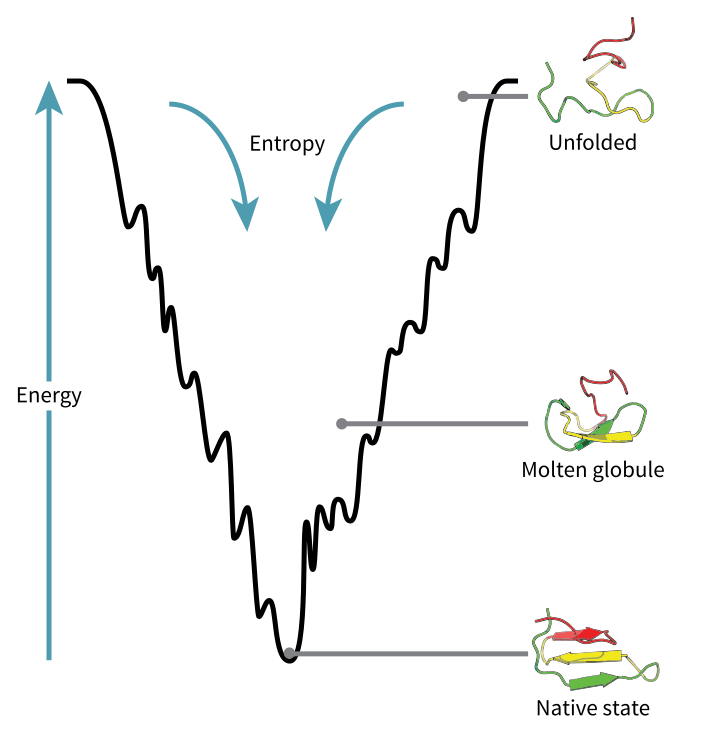
\includegraphics[width=0.8\textwidth]{lectures/160606/pix/Folding_funnel_schematic.png}


In der Natur falten Proteine aber im Bereich von Millisekunden. Wie ist das zu erklären?\newline
Lokale Interaktionen führen den Faltungsprozess und schränken die Möglichkeiten ein.
Experimente zeigen die resultierenden Intermediates und Transition states.\newline
Struktur und Faltung sind also \emph{sequenzkodiert}.
\subsection{Protein-Domains (Domänen)}
\begin{itemize}
 \item Protein-Untereinheit
 \item Falten unabhängig vom Rest des Proteinstrukturen
 \item Meistens funktionelle Untereinheit
 \item ca. 2700 Familien
 \item ca. 120000 Proteine (pdb)
 \item ca. 2/3 sind Multidomain-Proteine
 \item ca. 1224 Folds
 \begin{itemize}
  \item Folds (SCOPe-Datenbank) Structural classification of proteins
  \item All $\alpha$
  \item All $\beta$
  \item $\alpha / \beta$, abwechselnde $\alpha/ \beta \Rightarrow$ parallele $\beta$-Faltblätter
  \item $\alpha + \beta$, getrennte $\alpha, \beta \Rightarrow$ antiparallele $\beta$-Faltblätter
  \item Multidomain ($\alpha + \beta$)
  \item Andere (coiled coil, membrane, cell-surface)
  \end{itemize}
\end{itemize}
\subsection{Zwei Typen von Vorhersagen}
\begin{itemize}
 \item Ab initio
 \item Template based
 \begin{itemize}
  \item Homology based
  \item Threading
 \end{itemize}
\end{itemize}
\subsubsection{Ab-initio-Vorhersage}
\begin{itemize}
 \item Suche Strukturvorschläge
 \item Bewerten der Strukturen
 \begin{itemize}
 \item physikalisch
 \item knowledge-based $log(\frac{observed}{expected})$
\end{itemize}
\end{itemize}
\paragraph{Physikalisch}
Molecular force field
\paragraph{E\textsubscript{Bindung}}
\begin{itemize}
 \item Bindungen
 \begin{itemize}
  \item Abstand
  \item Winkel $\alpha$ (Bindung)
 \end{itemize}
 \item Winkel $\phi$ (Torsion)
\end{itemize}
\paragraph{E\textsubscript{ungebunden}}
\begin{itemize}
  \item Ladungen
  \item Dipol
\end{itemize}
 $E=E_{Bindung} + E_{Nicht-Bindung}$
 
 $E_{Bindung} = \sum\nolimits_{\alpha} k(\alpha - \alpha_0)^2 \\
 + \sum\nolimits_{Bindungen} k (r - r_0)^2$ \\ 
 + $\sum\nolimits_{\phi (Torsion)} \frac{V_n}{2} (1 - \cos(n\phi - \gamma))$\\
 Alternative für Bindungspotential (Morse-Potential\footnote{\url{https://en.wikipedia.org/wiki/Morse_potential}})
 $\sum\nolimits_{Bindungen} D_e * (1 - e^{-a(r-r_0)^2})$
 
\begin{description}
  \item [$k$] Kraftkonstante
  \item [$\alpha$] Bindungswinkel
  \item [$r$] Bindungslänge
  \item [$r_0$] Bindungslänge mit der geringsten potentiellen Energie
  \item [$D_e$] Dissoziationsenergie
  \item [$a = (0.5 * \frac{k}{D_e})^{1/2}$] ``Steifigkeits-''Konstante
  \item [$V_n$] Barrier height
  \item [$\gamma$] Phasenverschiebung
\end{description}

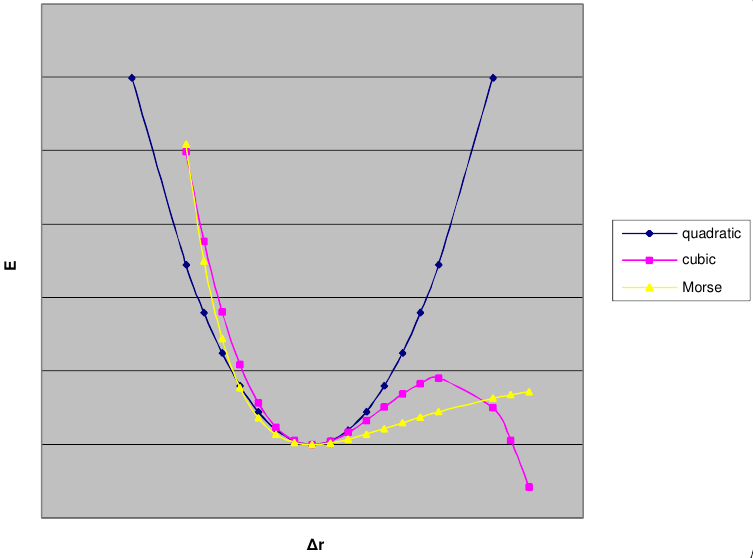
\includegraphics[width=0.8\textwidth]{lectures/160606/pix/potential_function.png}\\

$E\textsubscript{Nicht-Bindung} = $
\begin{description}
 \item [$\sum\nolimits_{i,j \in Atome} \frac{P_i P_j}{\epsilon r_{i,j}}$] Ladung: Coulomb-Terme
 \item [$+ \sum_{Paar} \frac{c}{r^{12}} - \frac{c}{r^6}$] Dipol: Van-der-Waals-Kräfte, Lennard-Jones-Potential 12, 6
\end{description}

cut-off-radius

\paragraph{Lösungsmittel}
\begin{itemize}
 \item implicit solvent
 \item explicit solvent
\end{itemize}
Spezialterme: H-Terme, $\Pi$-Interaktionen
\paragraph{Knowledge based}
\begin{itemize}
 \item coarse-graining
 \item c\textsubscript{$\alpha$} als Beschreibung der AS
 \item Alle Backbone-Atome
 \item Alle Backbone-Atome + repräsentativ die Sk (center of mass)
 \item Alle Atome
\end{itemize}

\paragraph{Einfache Potentiale}
\begin{itemize}
  \item Abstand der Aminosäuren
  \item Nachbarschaft der Aminosäuren
\end{itemize}

\paragraph{QUARK}
\begin{itemize}
  \item Backbone atomweises Paar-Potential
  \item Sk-Schwerpunkt
  \item Excluded volume
  \item H-Bindungen
  \item Surface accessible area
  \item Torsionswinkel im Backbone
  \item Distanzen von Fragmenten
  \item Gyrationsradius
  \item $\beta \alpha \beta$-linkshändig (HIER FEHLT NOCH WAT)
  \item $\beta \alpha \beta$-packing
  \item $\alpha$-packing
  \item $\beta$-packing
\end{itemize}

Konformation $\Rightarrow$ dafür Minimum
\begin{itemize}
 \item Steepest descent
 \item Conjugate gradient
 \item Newton-Verfahren
\end{itemize}

\begin{itemize}
 \item Monte-Carlo-Verfahren
 \item Simulated annealing
\end{itemize}

\subsubsection{Template based methods}
\paragraph{Homology based}
\begin{itemize}
 \item Sequenzalignment zu den Sequenzen der bekannten Strukturen
 \item Alignment der Sequenz zur Struktur des Kandidaten
 \item Bauen einer Struktur aus dem Alignment
 \item Bewerten der Struktur
\end{itemize}

HIER FEHLT EIN BILDCHEN

\begin{itemize}
 \item Verbinden der Distanzpotentiale (gewichtet, multiplikativ)
\end{itemize}
CASP (critical assessment of structure prediction)

\paragraph{Threading}
\begin{enumerate}
  \item Sequenz-Struktur-Alignment zur Identifizierung der Kandidaten\\
  $\left(\begin{array}{c} \alpha \\ 0.5 \\ P \\ groß \end{array}\right)$
  $\left(\begin{array}{c} \alpha \\ 0.3 \\ P \\ klein \end{array}\right)$
  \item Bauen einer Struktur aus Alignment
  \item Bewerten der Struktur
\end{enumerate}